
%
% Gas Target NIM Paper 
%
% Updated 22 October 2018 by Natalie and merged
%

%\documentclass[preprint,12pt]{elsarticle}

%% Use the option review to obtain double line spacing
%% \documentclass[authoryear,preprint,review,12pt]{elsarticle}

%% Use the options 1p,twocolumn; 3p; 3p,twocolumn; 5p; or 5p,twocolumn
%% for a journal layout:
%% \documentclass[final,1p,times]{elsarticle}
%\documentclass[final,1p,times,two]{elsarticle}
%% \documentclass[final,3p,times]{elsarticle}
%% \documentclass[final,3p,times,twocolumn]{elsarticle}
%% \documentclass[final,5p,times]{elsarticle}
\documentclass[final,5p,times,twocolumn,balance]{elsarticle}

%% For including figures, graphicx.sty has been loaded in
%% elsarticle.cls. If you prefer /to use the old commands
\usepackage{amsmath, amssymb, amsfonts, latexsym}
\usepackage{epsfig}
\usepackage{subcaption}
\usepackage{adjustbox}
\usepackage{mathtools}
\usepackage{amssymb}
\usepackage{xcolor}
\usepackage{textcomp}
\usepackage{graphicx}
\usepackage{balance}
%\usepackage[LGRgreek]{mathastext}

%% The amsthm package provides extended theorem environments
%% \usepackage{amsthm}

%% The lineno packages adds line numbers. Start line numbering with
%% \begin{linenumbers}, end it with \end{linenumbers}. Or switch it on
%% for the whole article with \linenumbers.
%% \usepackage{lineno}

\journal{Nuclear Instruments and Methods}

\begin{document}

\begin{frontmatter}

%% Title, authors and addresses

%% use the tnoteref command within \title for footnotes;
%% use the tnotetext command for theassociated footnote;
%% use the fnref command within \author or \address for footnotes;
%% use the fntext command for theassociated footnote;
%% use the corref command within \author for corresponding author footnotes;
%% use the cortext command for theassociated footnote;
%% use the ead command for the email address,
%% and the form \ead[url] for the home page:
%% \title{Title\tnoteref{label1}}
%% \tnotetext[label1]{}
%% \author{Name\corref{cor1}\fnref{label2}}
%% \ead{email address}
%% \ead[url]{home page}
%% \fntext[label2]{}
%% \cortext[cor1]{}
%% \address{Address\fnref{label3}}
%% \fntext[label3]{}

\title{Density Changes in Low Pressure Gas Targets for Electron Scattering Experiments}
%\title{Performance of the Hall A Tritium Target}

\author[Kent]{Sheren Alsalmi}
\author[UNH]{Nathaly Santiesteban}
\author[UNH]{Shujie Li}
\author[Kent]{Tong Su}
\author[JLab]{David Meekins}

\address[Kent]{Kent State University, Kent, OH 44240}
\address[UNH]{University of New Hampshire, Durham, NH 03824}
\address[JLab]{Jefferson Lab, Newport News, VA 23601}

\begin{abstract}
The Jefferson Lab target group has developed closed gas target cells for use in electron scattering experiments. This system was initially developed for the safe use of tritium gas, but can be used with a wide variety of gases.  Thus far the system has been used in the 12 GeV 
era of experiments of the Continuous Electron Beam Accelerator Facility (CEBAF) using $^{3}$H, $^{3}$He, $^{2}$H, $^{1}$H and $^{40}$Ar with nominal beam currents of  $22.5$ $\mu A$.  The target cells are machined from solid  aluminum blocks, they have an active region of $25$ $cm$ long with a $1.3$ $cm$ diameter with approximately $0.25$ $mm$ thick windows for the beam entrance and exit.   While the fill density of the cells is known, the density of the gas when heated by the electron beam needs to be determined in order to extract experimental cross sections using these target cells. We find the density of the target dependent on the current of the electron beam going through the cell. In this study, the expression to calculate the percentage of density changed for any current within the range of $2.5$ to $22.5$ $\mu A$ is obtained for each target.
 


  
\end{abstract}

\begin{keyword}
Density \sep target system
\sep $^{3}$H, $^{3}$He, $^{2}$H, $^{1}$H, $^{40}$Ar
\sep CEBAF
%% keywords here, in the form: keyword \sep keyword
%% PACS codes here, in the form: \PACS code \sep code
%% MSC codes here, in the form: \MSC code \sep code
%% or \MSC[2008] code \sep code (2000 is the default)
\end{keyword}
\end{frontmatter}

%% \linenumbers

%% main text
\section{Introduction}
\label{}
%%%%%

The tritium target was developed in Hall A at Jefferson Lab for the experiments E12-10-103 (MARATHON) \cite{marathon}, E12-11-112 ($x_{b}>1$) \cite{E12-11-112}, E12-14-011 ($e'p$) \cite{E12-14-011}, E12-17-003 (Hypernuclear) \cite{hypernuclear} and E12-14-009 (elastic) \cite{E12-14-009}. This target system was first used by the experiment E12-14-012 (Argon) \cite{E12-14-012} during spring of 2017, and it was later used by the tritium set of experiments during  Fall 2017 and  2018 year. 

The goal of the target system was to build a simple and robust structure to contain the optimal amount of tritium, and to minimize 
its hazards. There were several requirements in order to achieve a safe tritium target system, and this paper summarizes the main characteristic 
of its design, development and results. 

In addition to the hardware development, this paper also aims to present the density fluctuations of the four different gasses used 
with the target system, $^{3}$H, $^{3}$He, $^{2}$H, $^{1}$H and $^{40}$Ar when the beam hits the targets. The current in the target 
increases the temperature, therefore the density of the gasses are changed. The goal is to determine a functional form of the density 
change for any given current, which will be in the analysis of all the experiments in order to calculate the correct luminosity.

The data for the density analysis was taken with the Left High Resolution Spectrometer (LHRS) at Hall A during February 2017 
for the $^{40}$Ar target and during December 2017 for the other targets. The beam energy for the study was $2.2$ GeV in all 
cases, and the momentum and angle were $17.5 ^\circ $ and $1.79$ GeV for $^{40}$Ar, and $17.0 ^\circ $ and $1.99$ GeV for 
the other targets.

The target system is summarized, followed by the description of the process to calculate the density change, including 
some revelant hardware and calibration devices in the analysis, as well as the systematics . Finally, a quadratic functional form 
to calculate the percentage of density changed with respect to the current is  obtained for each target.


\section{Target System}

A modular design was used for the target ladder in order to install the tritium cell after all the other targets were placed. 
Particularly, the tritium cell was the only cell that was not filled onsite at Jefferson Lab. It was filled at the Savannah River 
site Tritium Enterprises (SRTE), and it was shipped in a dual vessel, in order  to determine if the cell failed without having to
open the container. The container was located in Hall A at all time in Jefferson Lab, with only qualified personal access. The cell only was out of the container while it was inside the scattering chamber. 

\begin{figure}[htbp]
\centering
  % Se pueden incluir figuras jpeg al compilar con PDFLatex
  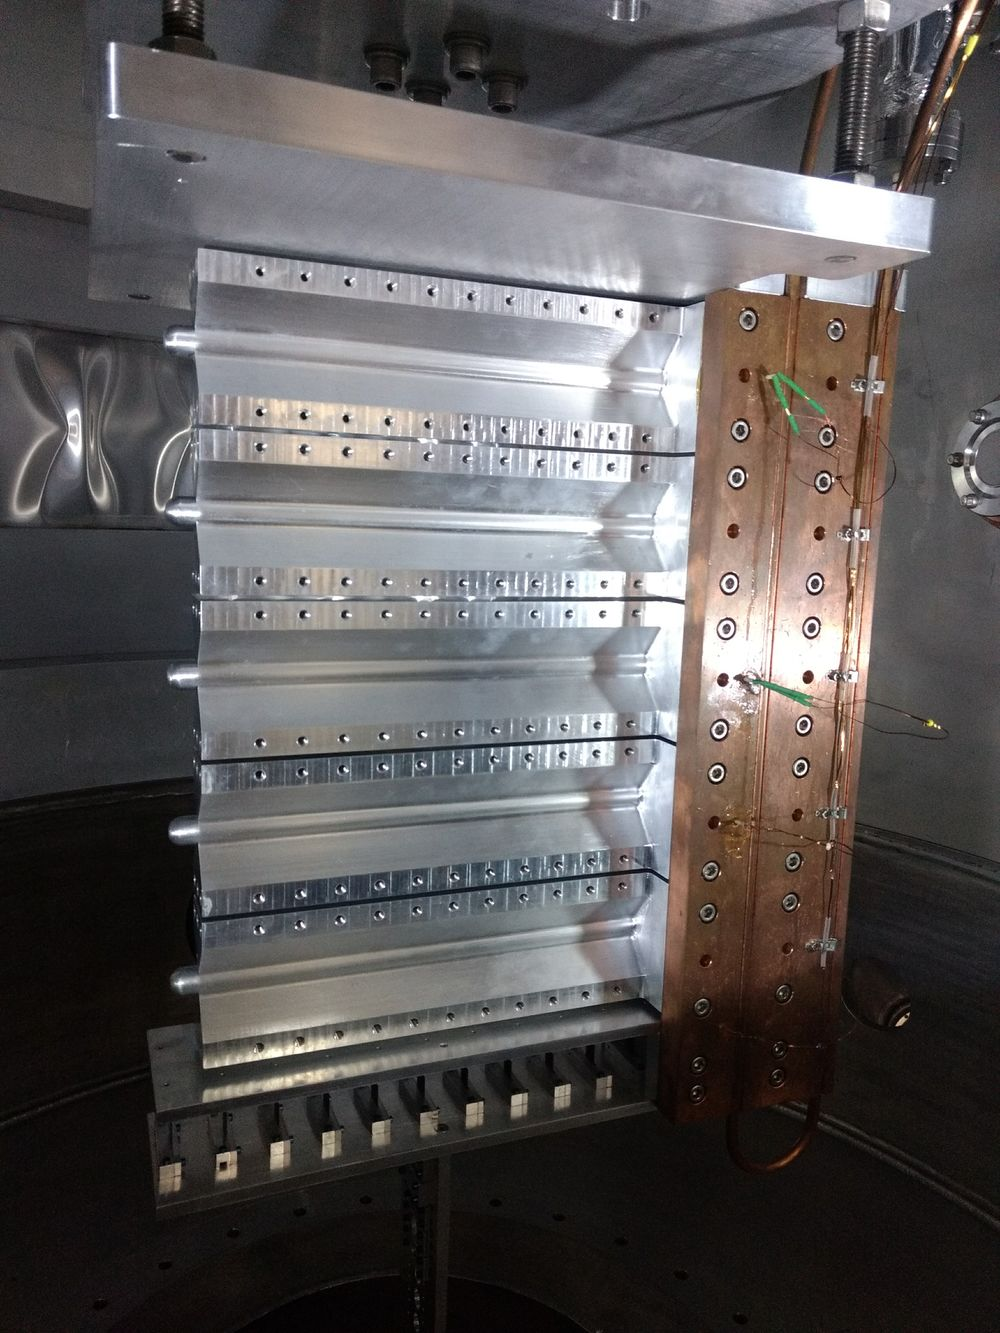
\includegraphics[width=6.5cm]{images/ladder.jpg}\\
  \caption{Ladder Assembly. Five cells were assembled during Fall 2017 to Spring 2018, $^{3}H$, $^{2}H$, $^{1}H $, $^{3}He$ and empty cell from top to bottom
 }\label{ladder}
\end{figure}

The target ladder allows a total of five cells and it is shown in Figure \ref{ladder}.  The bottom cell is an empty cell used for background measurements. The tritium group of experiments cycled between the $^{3}$H, $^{2}$H, $^{1}$H, $^{3}$He target cells for most of the beam time. The only gas target used in February 2017 was $^{40}$Ar.

The vacuum system of the target provided containment and confinement during normal operations. This system includes the scattering chamber, 
the pumping system, the upstream beam isolation window and the beam dump line.  

The scattering chamber has a volume of about 1900 liters and its configuration has been used in Hall A for more than 15 years. 
In this particular set of experiments, the chamber has an extra beryllium (99.8$\%$) window to separate the upstream beamline 
and the scattering chamber. The window contains a collimator to minimize beam scraping on the target cell walls. Furhermore, 
the downstream beam dump line was isolated from the scattering chamber using a gate valve during installation, maintenance and removal operations of the target cells. 

In addition, a special exhaust system was built to remove tritium from the scattering chamber and/or Hall A in a controlled manner 
in case the the tritium containment systems failed. A temporary isolation room fixed to the scattering chamber, known as 
the transfer hut, was also directly attached to the scattering chamber during instalation. The scattering chamber was connected directly to the exhaust system. Thus, the air pulled through the hut into the chamber went directly through the exhaust system.  


\subsection{Target Cell Characteristics}

The entire target assembly was cooled with $15K$ helium from the Jefferson Lab End Station Refrigerator (ESR). The $15K$ helium was preheated to $40K$ and used to cool a heat sink attached to the cell assemblies. This removed about $15W$ of heat that is generated by the electron beam. 
The beam current allowed on the tritium cell was limited to a maximum of $22.5$ $\mu A$ \cite{engreport}.

The heat generated by the tritium decay is very small, about $50$ $mW$. The power deposited in the windows and gas is also relatively 
small with a beam current of $22.5$ $\mu A$. There was a deposited power of approximately $4.7$ $W$ in the entrance window, $5.1$ $W$ 
in the exit window, $3.8$ $W$ in the tritium gas, approximately $8.6$ $W$ in the hydrogen, deuterium and helium gases \cite{celldes}.
 
The filling parameters for each cell are summarized in Table \ref{tab:fill_tar} at room temperature. The target thickness values of this table are changed with the bean current and ultimately the percentage changed in the density will be applied as a correction factor to this values. The gas with major density used in the experiments was $^{40}$Ar and the lower density target was $^{3}H$.  Additionally, the top view of the cell is shown in Figure \ref{fig:cellconfig},  it shows the beam direction and the two windows of the cell.

\begin{table}[!h]
\centering
\begin{adjustbox}{width=0.5\textwidth}
\begin{tabular}{|c|c|c|c|c|}
\hline
Target   & Mass $(g)$           & \begin{tabular}[c]{@{}c@{}}$\rho t$ $(mg/cm^{2})$\\ Target thickness\end{tabular} & \begin{tabular}[c]{@{}c@{}}Filling Pressure\\ ($psia$) \end{tabular} & Temperature $(K)$  \\ \hline
$^{40}$Ar  & $1.943$              & $1455$                                           & $500$ & $291$ \\ \hline
$^{3}$H  & $0.102$              & $77 \pm 0.01$ & $203$                                                             & $291$\\ \hline
$^{3}$He & $ 3.01 \times 10^{-5}  $  & $53.4 \pm 0.6$ & $252.7$                                                           & $294.3$ \\ \hline
$^{2}$H  & $3.20\times10^{-5}$ & $142.2 \pm 0.8$  & $514.7$                                                           & $296.1$
\\ \hline
$^{1}$H  & $9.47 \times 10^{-6} $ & $70.8 \pm 0.4$  & $514.7$                                                          & $297.4$
\\ \hline
\end{tabular}
\end{adjustbox}
\caption{Gas target filling parameters. Temperatures have an uncertainty of $0.1\circ $. $^{40}$Ar taken from \cite{ar_config} and for the other targets from \cite{cellconfig}. }. 
\label{tab:fill_tar}
\end{table}

\begin{figure}[!h]
\centering
  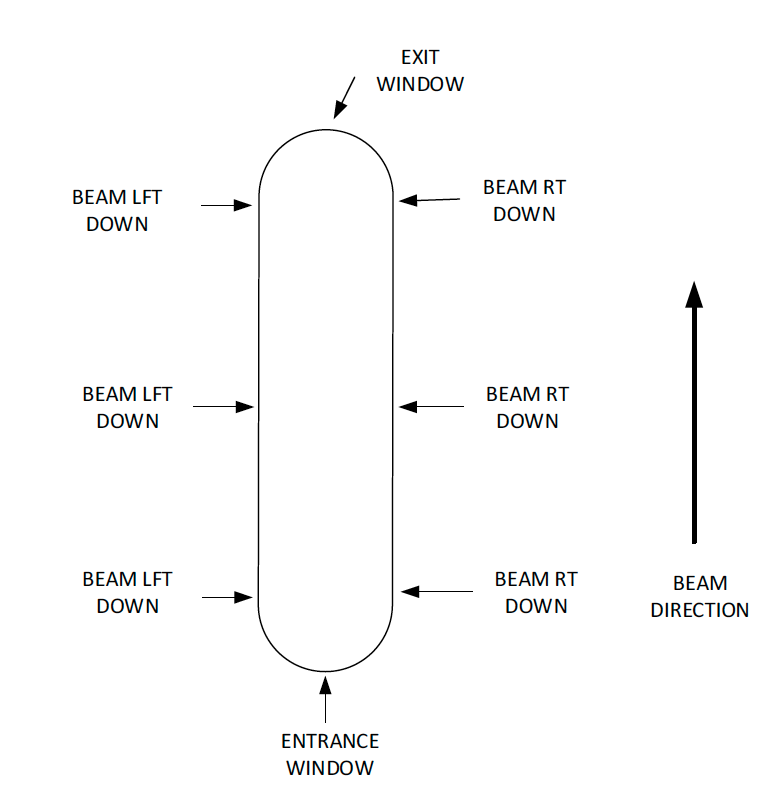
\includegraphics[width=\linewidth]{images/tgt_measurements.png}\\
  \caption{Measurement locations on the cells \cite{cellconfig}. 
 }\label{fig:cellconfig}
\end{figure}

The gas targets are contained in a $25$ $cm$ long by $1.3$ $cm$ diameter aluminum (7075-T6) sealed system, the target cell is shown in Figure \ref{cell}. 
The alloy 7075-T6 was chosen since it has high thermal conductivity, high yield strength, and it is used for target cells at JLab commonly. 
The windows for beam entrance and exit were designed to be $0.0254$ $cm$ and $0.0279$ $cm$ thick, respectively \cite{celldes}. However, due to the fact that the cell was machined out of a single aluminum piece, the exit window has slightly different measurements for each target, as it is summarized in Table \ref{tab:cell}.

The $^{40}$Ar cell was used in February 2017, and after the experiment finished, the cell was reused as the dummy cell for the tritium set of experiments. Table \ref{tab:cell} shows the $^{40}$Ar and the Dummy Cell as a single one. $^{40}$Ar experiment did not have a dummy cell, instead, it used two aluminum foils with in order to calculate the background contamination in the gas.

\begin{table*}[!h]
\centering
\begin{adjustbox}{width=1\textwidth}
\begin{tabular}{|c|c|c|c|c|c|}
\hline
Cell Position        & \begin{tabular}[c]{@{}c@{}} $^{40}$Ar/Dummy Cell\\ Thickness $(mm)$\end{tabular} & \begin{tabular}[c]{@{}c@{}}$^{3}H$ Cell\\ Thickness $(mm)$\end{tabular} & \begin{tabular}[c]{@{}c@{}}$^{1}H$ Cell\\ Thickness $(mm)$\end{tabular} & \begin{tabular}[c]{@{}c@{}}$^{2}H$ Cell\\ Thickness $(mm)$\end{tabular} & \begin{tabular}[c]{@{}c@{}}$^{3}He$ Cell\\ Thickness $(mm)$\end{tabular} \\ \hline
Entrance               &      $0.254 \pm 0.0051$                                                  & $0.253 \pm 0.004$                                                     & $0.311 \pm 0.001$                                                     & $0.215 \pm 0.004$                                                     & $0.203 \pm 0.007$                                                      \\ \hline
Exit                    &    $0.279 \pm 0.0051$                                                  & $0.343 \pm 0.047$                                                     & $0.330 \pm 0.063$                                                     & $0.294 \pm 0.056$                                                     & $0.328 \pm 0.041$                                                      \\ \hline
Exit left              &      $0.406 \pm 0.0051$                                                 & $0.379 \pm 0.007$                                                     & $0.240 \pm 0.019$                                                     & $0.422 \pm 0.003$                                                     & $0.438 \pm 0.010$                                                      \\ \hline
Exit right              &       $0.421 \pm 0.0051$                                                 & $0.406 \pm 0.004$                                                     & $0.519 \pm 0.009$                                                     & $0.361 \pm 0.013$                                                     & $0.385 \pm 0.016$                                                      \\ \hline
Mid left             &        $0.457 \pm 0.0051$                                                  & $0.435 \pm 0.001$                                                     & $0.374 \pm 0.004$                                                     & $0.447 \pm 0.009$                                                     & $0.487 \pm 0.060$                                                      \\ \hline
Mid right             &        $0.432 \pm 0.0051$                                                  & $0.447 \pm 0.004$                                                     & $0.503 \pm 0.005$                                                     & $0.371 \pm 0.012$                                                     & $0.478 \pm 0.007$                                                    \\ \hline
Entrance left      &          $0.508 \pm 0.0051$                                                  & $0.473 \pm 0.003$                                                     & $0.456 \pm 0.010$                                                     & $0.442 \pm 0.005$                                                     & $0.504 \pm 0.003$                                                      \\ \hline
Entrance right     &		 $0.424 \pm 0.0051$                             & $0.425 \pm 0.003$                                & 
$0.457 \pm 0.006$                                & 
$0.332 \pm 0.011$                                & 
$0.477 \pm 0.011$                                 \\ \hline
\end{tabular}
\end{adjustbox}
\caption{Cell wall thickness measurements for all the gas targets. Ar taken from \cite{ar_config} and for the other targets from \cite{cellconfig}.}
\label{tab:cell}
\end{table*}


\begin{figure*}[!h]
\centering
  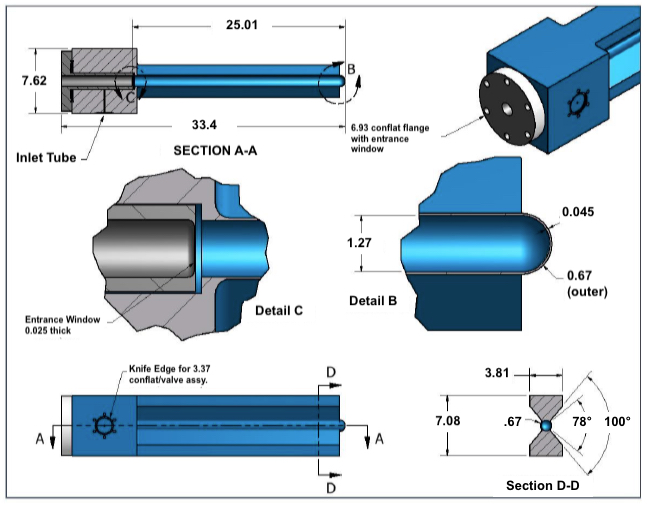
\includegraphics[width=13cm]{images/tritium_cell.jpg}\\
  %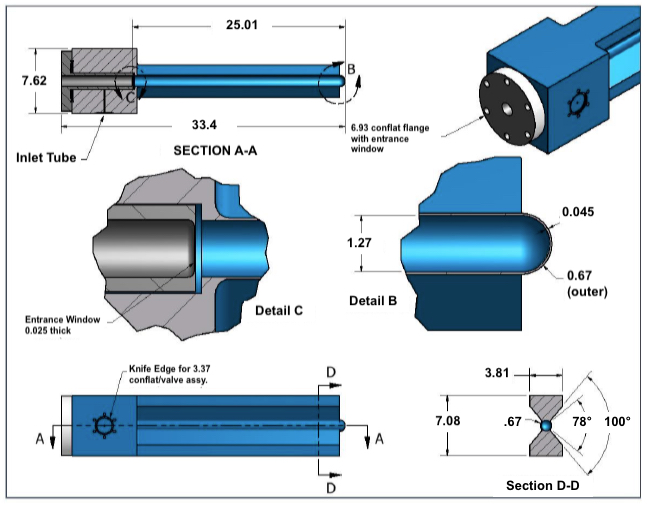
\includegraphics[width=\linewidth]{images/tritium_cell.jpg}\\
  \caption{Engineering design of an individual tritium gas target cell \cite{celldes}, using $cm$ units.
 }\label{cell}
\end{figure*}


\section{Experimental Hall A}

The data was taken with the LHRS. The basic components of the LHRS are
one non superconducting quadrupole(Q1),two superconducting quadrupoles (Q) and one superconducting dipole (D) in a Q1QDQ configuration. The quadrupoles align the electron while the dipole determines the momentum of the electrons that get to the detectors.

After passing the magnets, the scattered electrons go through two Vertical Drift Chambers (VDCs), where the electrons ionize the gas inside the chambers. Wi9ith the information the position and angle of the trajectory are found. Then, the trigger scintillators s0 and s2, with the Cherenkov detector filled with CO2 between the trigger scintillator planes are found. They identify the electrons with $99 \%$  efficiency and the threshold for pions is $4.8$ $GeV$ . Finally, the preshower and shower lead glasses blocks induce a cascade of pair production and bremsstrahlung radiation from energetic particles, which are used for the measurement of the energy of the electrons \cite{Alcorn:2004sb}.


\section{Beam Current Monitor (BCM)}
\label{BCM}

The Beam Current Monitor (BCM) is the highest source of systematic uncertainty in the density study. The BCM system consists of a toroidal sensor (Unser), an RF cavity in the upstream side and an RF cavity in the downstream side of the Unser, and a data-acquisition system.  

The Unser has a sensitivity of $4$ $mV/\mu A$ \cite{denard}, with an offset that drifts over time. The large offset noise vetoes the possibility of use the Unser during all the measurements. Therefore, the Unser is an absolute measurement of the current that is used to calibrate the cavities. These calibrations are required periodically.

The Unser monitor is composed of two identical toroidal cores driven in opposite ways by an external source.  The DC component of the current flowing through the toroid sensor is detected by a magnetic modulator. The beam current in the cores produces a flux imbalance, which generates an output signal proportional to the even harmonics of the frequency of excitation, In the absence of DC current, the sum of the signals is zero \cite{denard}. The Unser is calibrated by sending a known DC current through the wire that passes inside of the toroids with a current source.  


\begin{figure}[!h]
    \centering
    \includegraphics[width=\linewidth]{images/unser_calibration.pdf}
    \caption{Wire Unser calibration. The band reprecents the $95$ $\%$ confidence level of the linear fit.}
    \label{fig:unser_cal}
\end{figure}
  
\begin{figure}[!h]
      \centering
    \includegraphics[width=\linewidth]{images/dnew_calibration.pdf}
    \caption{BCM calibration. The band reprecents the $95$ $\%$ confidence level of the linear fit.}
    \label{fig:dnew_cal}
\end{figure}

Two stainless steel resonant cavities surround the Unser and are tuned to the frequency of the beam $1.497$ $GHz$ with a quality coefficient $Q \approx 500$.    The cavities are composed of loop antennas located where the magnetic field is maximum. When the beam passes through, the output RF signal is proportional to the current \cite{denard}. As consequence, the BCM response is linear with respect to the current. In the BCM calibration, the accelerator sent a set of currents, the absolute value of the current is measured with the Unser and its values are used to calculate the linear dependence of the BCM.


Figure \ref{fig:unser_cal} shows the Unser calibration, the gain of the Unser is $0.0002497 \pm 9.6 \times 10^{-7} $ $\mu A/Hz$. Over time, the Unser gain has shown to be stable within $0.1$ $\%$ of $4$ $mV/\mu A$. 

The beam current was calculated using the gain of the Unser, this current was used for the calculation of the linear parameters of the BCM linear response, as it is shown in Figure \ref{fig:dnew_cal}. In general, the beam current can be calculated using,

\begin{equation}
I = g_{BCM}\cdot f+O
\label{eq:current_calc}
\end{equation}

\noindent where $g_{BCM}$ and $O$ are the fit parameters, which correspond to $0.0003264 \pm 1.4 \times 10^{-6}$ $\mu A/Hz$ and $0.1 \pm 0.09$  $\mu A$, respectively. Finally, for any given 
frequency $f$, the current $I$ is given by Equation \ref{eq:current_calc}.

\section{Method Overview}

The density of the target is known when it is filled, but simulations have shown that the beam current will change the density of the target. This effect is directly related with the luminosity, and therefore with any cross section measurement \cite{celldes}. It is expected that the density remains stable if the current applied to the gas is constant, when it reaches equilibrium. The production currents for the experiments were $10$ $\mu A$ and $22.5$ $\mu A$, therefore, the goal is to calculate the density of the targets at those currents.  

In order to measure the density change, the charge normalized Yield is measured for different currents. After the charge Yield is calculated, it is normalized with respect to the lowest current point, and finally it is assumed when there is not current, the charge normalized Yield is $1$. The percentage changed in the normalized Yield corresponds to the percentage of density changed in the target. 

The charge normalized Yield is given by 

\begin{equation}
Y = \frac{PS \cdot N}{ Q \cdot \epsilon \cdot LT }
\label{eq:yield}
\end{equation}

\noindent where $N$ is the number of good electrons, $PS$ is the prescale factor, $Q$ is the charge, $\epsilon $ is the combined efficiencies of detectors, triggers and events selection cuts and $LT$ is the live-time. Each one of these parameters is explained in detail in the following sections.

\subsection{Events Selection}
In order to extract a good electron sample, several cuts were applied to the data. These cuts can be summarized in two groups: Acceptance Cuts, which assure that the events are selected within the spectrometer specifications, and Particle IDentification (PID) Cuts, which focus in the selection of electrons scattered from the gas target. 

\begin{itemize}
\item[i.]Acceptance cuts include the momentum acceptance $dp$ and the angular resolution, the out-of-plane angle $\theta $ and the in-plane angle $\phi $. Specifically, the range used in the study 
are $|dp| < 4.5$ $\%$,  $|\theta| < 30 $ $mrad  $ and $|\phi| < 25$ $mrad$.

\item[ii.] The trigger selected required both scintillator planes and the Cherenkov detector to fire, in order to exclude pions events, and reduce the dead-time.

\item[iii.] It was  probed through the course of this study that as long as the sample of electrons is chosen consistently, the results will remain invariant within $1$ $\%$.

\item[iv.] The gas events selected were in a range of $16$ $cm$ with respect to the center of the target. The endcaps were removed in order to keep the background as low as possible.

\end{itemize}

\subsection{Efficiencies Estimations } 

The efficiencies incorporated in this study include the detectors and trigger capabilities of measurement, and the cuts effects. 

Only electrons with one track in the VDC were selected. Therefore, the ratio between the total of particles with one track with respect to the total number of particles (including multi track and non track particles) corresponds to the VDC efficiency.  

The trigger efficiency was calculated using other trigger type, where only both scintillators were used to record the events. In this sense, the difference between the main trigger and the efficiency trigger is the Cherenkov detector.  The ratio between the events recorded with the main and the efficiency trigger corresponds to the trigger efficiency.

The Cherenkov efficiency was calculated by selecting a clean sample of electrons detected in the Calorimeters detectors, and counting the number of events that also were detected in the Cherenkov detector.

The Calorimeters efficiency was measured by selecting a clean sample of electrons in the Cherenkov detector and counting the number of electrons that also fired the Calorimeters.



\subsection{Live-Time Calculation } 

The live-time is related with the limitation of the speed of DAQ system to record events onto the hard disk. It is dependent on the electronics, computers and trigger rate and is calculated using the ratio between the number of events recorded over the total number of events seen by the trigger. 



\subsection{ Total Charge}

The beam is not completely stable in all the run, it may trip or fluctuate overtime. Therefore, the number of events and the charge is calculated only if the average current is within a window of $\pm 2$ $\mu A$ of the current asked to the accelerator.  The charge is calculated using the BCM calibration (See Section \ref{BCM}) result integrated over time.


\section{Solid Target Check}

The aim of the analysis is to measure the density change when the beam is on the gas targets using the Yield analysis. In order to test the method, the same analysis is implemented in a solid target, in particular, in the $^{40}$Ar experiment using a carbon foil, and in the Tritium experiment using an aluminum target. When a solid target is used, the density does not vary and therefore, the Yield should be constant for any given current.

\begin{figure}[htbp]
    \centering
    \includegraphics[width=\linewidth]{images/solid_target.pdf}
    \caption{$Al$ Yield analysis for the tritium set of experiments.}
    \label{fig:solid}
\end{figure}

Figure \ref{fig:solid} show the Normalized Yield of the solid target. The charge Yield was calculated using Equation \ref{eq:yield} for the the different beam currents and it was normalized with respect to the lowest current Yield value The plot shows that the Yield did not change within about $0.5 \%$. A zeroth order and a first order polynomial were used to fit the data, with a $\chi ^{2}$ of $1.93$ and $0.38$, respectively. As a result, for a solid target, the charge Yield is independent of the current since the density of the target remains constant.

\section{Background Contamination}

The aluminum windows of the target cell contribute in the Yield calculation of the gas targets. Therefore, dummy cell measurements with aluminum foils of identical properties of the end-caps of the gas targets for the $^{40}$Ar target, and with a dummy cell for the other targets were taken, in order to remove the background events coming from the aluminum and from rescattered particles inside of the spectrometer. 

In order to check how end-cap background changes with increasing current, a comparison between the background at low and high current was measured for the dummy targets. The charge yield given by Equation \ref{eq:current_calc} was calculated along the target length, and the ratio of the events at high current to low current was estimated. The ratio was found to be 1.006, which indicates that the windows background will not increase with increasing current, as is expected for a solid target. 

\begin{figure}[h]
 \centering
 \includegraphics[width=\linewidth]{images/contamination.pdf}
  \caption{Background contamination spectrum of the dummy target compared with a tritium gas run at $2.5$ $\mu A$.}
  \label{fig:bk_empty}
\end{figure}

Figure \ref{fig:bk_empty} shows the spectrum of the charge normalized yield for dummy cell and the tritium gas, for a beam current of $2.5$ $\mu A$. In this analysis, the density study was done in a symmetric region of $16$ cm around the center of the target, therefore, the percentage of background events coming from the aluminum end-caps is given by the ratio between the charged yield of the empty cell and the gas. Table \ref{tab:contamination_al} summarizes the percentage of contamination in the gas targets for the different currents used in the study. Note that the currents correspond to the values asked to the accelerator as a simplification, the measured current for each run is slightly different, due to the normal operation of the accelerator.
 
\begin{table}[h!]
\begin{tabular}{|c|c|c|c|c|c|c|}
\hline
\textbf{\begin{tabular}[c]{@{}c@{}}Current \\ $(\mu A)$\end{tabular}} & \textbf{\begin{tabular}[c]{@{}c@{}}$^{3}H$\\ (\%)\end{tabular}} & \textbf{\begin{tabular}[c]{@{}c@{}}$^{3}He$\\ (\%)\end{tabular}} & \textbf{\begin{tabular}[c]{@{}c@{}}$^{2}H$\\ (\%)\end{tabular}} & \textbf{\begin{tabular}[c]{@{}c@{}}$^{1}H$\\ (\%)\end{tabular}} & \textbf{\begin{tabular}[c]{@{}c@{}}Current\\ $(\mu A)$\end{tabular}} & \multicolumn{1}{l|}{\textbf{\begin{tabular}[c]{@{}l@{}}Argon\\ (\%)\end{tabular}}} \\ \hline
2.5                                                              & 1.7                                                             & 1.6                                                              & 0.7                                                             & 1.1                                                             & 2.5                                                             & 0.3                                                                                \\ \hline
5                                                                & 1.7                                                             & 1.6                                                              & 0.7                                                             & 1.2                                                             & 4.5                                                             & 0.3                                                                                \\ \hline
10                                                               & 1.7                                                             & 1.7                                                              & 0.8                                                             & 1.2                                                             & 8                                                               & 0.3                                                                                \\ \hline
15                                                               & 1.8                                                             & 1.8                                                              & 0.8                                                             & 1.3                                                             & 12                                                              & 0.3                                                                                \\ \hline
22.5                                                             & 1.8                                                             & 1.8                                                              & 0.8                                                             & 1.3                                                             & 15                                                              & 0.3                                                                                \\ \hline
\multicolumn{5}{|l|}{}                                                                                                                                                                                                                                                                                                                    & 18                                                              & 0.3                                                                                \\ \hline
\end{tabular}
\caption{Aluminum windows contamination in a $16$ $cm$ range with respect to the center of the target, for the different currents Currents are different for $^{40}$Ar with respect to the other experiments.}
\label{tab:contamination_al}
\end{table}

 
\section{Gas Target Results}

The density change was measured by calculating the charge Yield for different currents. This yield is normalized with respect to the lowest current point. In the absence of beam current, the density corresponds to the filling density value, therefore, it is assumed that at $0$ $\mu A$ the normalized Yield is $1$, consequently, the points are extrapolated to this normalization value. 

Figures  \ref{fig:argon_data}, \ref{fig:tritium_data}, \ref{fig:helium_data}, \ref{fig:deuterium_data} and \ref{fig:hydrogen_data},  show the density  change for the different gas targets. Tthe density decreases with the intensity of the current and its behavior is approximated by a quadratic function,  

\begin{figure}[!h]
 \centering
 \includegraphics[width=\linewidth]{images/argon_data.pdf}
  \caption{$^{40}$Ar density analysis.}
  \label{fig:argon_data}
\end{figure}


\begin{equation}
f = a\cdot I^{2} + b \cdot {I} + c
\label{eq:boiling_factor}
\end{equation}

\noindent where $a$, $b$ and $c$ are the fit parameters, $I$ is the beam current and $f$ is equivalent to the factor that the density changed. Table \ref{tab:fit_parameters} shows the fit parameters for each target, which can be used to calculate the density change of the gas targets for any current in the range $0-22.5$ $\mu A$. The error bar in the plots represents the statistical values, and the fit was calculated with respect to those values. 




\begin{table}[!h]
\begin{tabular}{|c|c|l|c|c|l|}
\hline
\multicolumn{3}{|c|}{\textbf{$^{3}$H Fit Parameters}}                                & \multicolumn{3}{l|}{\textbf{$^{3}H$ Correlation Factors}}    \\ \hline
\textbf{a}              & \multicolumn{2}{c|}{$1.06e-04 \pm 3.6e-05$}                & \textbf{C(a, b)}             & \multicolumn{2}{c|}{$-0.974$} \\ \hline
\textbf{b}              & \multicolumn{2}{c|}{$-0.0068 \pm 8.9e-04$}                 & \textbf{C(b, c)}             & \multicolumn{2}{c|}{$-0.888$} \\ \hline
\textbf{c}              & \multicolumn{2}{c|}{$1. +/- 0.003$}                        & \textbf{C(a, c)}             & \multicolumn{2}{c|}{$0.801$}  \\ \hline
\multicolumn{3}{|c|}{\textbf{$^{3}$He Fit Parameters}}                               & \multicolumn{3}{c|}{\textbf{$^{3}He$ Correlation Factors}}   \\ \hline
\textbf{a}              & \multicolumn{2}{c|}{$1.036e-04\pm 2.5-05$}                 & \textbf{C(a, b)}                      & \multicolumn{2}{c|}{$-0.973$} \\ \hline
\textbf{b}              & \multicolumn{2}{c|}{$-0.0051 \pm 6.4e-04$}                 & \textbf{C(b, c)}                      & \multicolumn{2}{c|}{$-0.879$} \\ \hline
\textbf{c}              & \multicolumn{2}{c|}{$1 \pm 0.003$}                         & \textbf{C(a, c)}                     & \multicolumn{2}{c|}{$0.779$}  \\ \hline
\multicolumn{3}{|c|}{\textbf{$^{2}$H Fit Parameters}}                                & \multicolumn{3}{c|}{\textbf{$^{2}H$ Correlation Factors}}    \\ \hline
\textbf{a}              & \multicolumn{2}{c|}{$1.16e-04 \pm 2.9e-05$} & \textbf{C(a, b)}             & \multicolumn{2}{c|}{$-0.973$} \\ \hline
\textbf{b}              & \multicolumn{2}{c|}{$-0.0067 \pm 7.1e-04$}                 & \textbf{C(b, c)}             & \multicolumn{2}{c|}{$-0.895$} \\ \hline
\textbf{c}              & \multicolumn{2}{c|}{$1. \pm 0.003$}                        & \textbf{C(a, c)}             & \multicolumn{2}{c|}{$0.805$}  \\ \hline
\multicolumn{3}{|c|}{\textbf{$^{1}$H Fit Parameters}}                                & \multicolumn{3}{c|}{\textbf{$^{1}H$ Correlation Factors}}    \\ \hline
\textbf{a}              & \multicolumn{2}{c|}{$1.70e-04 \pm 4.7e-05$}                & \textbf{C(a, b)}             & \multicolumn{2}{c|}{$-0.978$} \\ \hline
\textbf{b}              & \multicolumn{2}{c|}{$-0.009 \pm 0.0012$}                   & \textbf{C(b, c)}             & \multicolumn{2}{c|}{$-0.881$} \\ \hline
\textbf{c}              & \multicolumn{2}{c|}{$1. \pm 0.006$}                        & \textbf{C(a, c)}             & \multicolumn{2}{c|}{$0.788$}  \\ \hline
\multicolumn{3}{|c|}{\textbf{$^{40}$Ar Fit Parameters}}                              & \multicolumn{3}{c|}{\textbf{$^{40}Ar$ Correlation Factors}}  \\ \hline
\textbf{a}              & \multicolumn{2}{c|}{$4.33 e-04 \pm 1.5e-04$}               & \textbf{C(a, b)}             & \multicolumn{2}{c|}{$-0.981$} \\ \hline
\textbf{b}              & \multicolumn{2}{c|}{$-0.021 \pm 0.003$}                    & \textbf{C(b, c)}             & \multicolumn{2}{c|}{$-0.942$} \\ \hline
\textbf{c}              & \multicolumn{2}{c|}{$1. \pm 0.02$}                         & \textbf{C(a, c)}             & \multicolumn{2}{c|}{$0.867$}  \\ \hline
\end{tabular}
\caption{Fit parameters obtained for the percentage of density change calculation with respect to the beam current.}
\label{tab:fit_parameters}
\end{table}




\begin{figure*}[h]
\begin{center}
  \begin{subfigure}{8cm}
    \centering\includegraphics[width=8cm]{images/tritium_data.pdf}
    \caption{$^{3}H$ Density Analysis. }
    \label{fig:tritium_data}
  \end{subfigure}\vspace{0.5cm}
  \begin{subfigure}{8cm}
    \centering\includegraphics[width=8cm]{images/helium_data.pdf}
    \caption{$^{3}He$ Density Analysis.}
    \label{fig:helium_data}
  \end{subfigure}\vspace{0.5cm}
  \begin{subfigure}{8cm}
    \centering\includegraphics[width=8cm]{images/deuterium_data.pdf}
    \caption{$^{2}H$ Density Analysis.}
    \label{fig:deuterium_data}
  \end{subfigure}
  \begin{subfigure}{8cm}
    \centering\includegraphics[width=8cm]{images/hydrogen_data.pdf}
    \caption{$^{1}H$ Density Analysis.}
    \label{fig:hydrogen_data}
  \end{subfigure}
  \end{center}
  \label{fig:tritium_targets}
  \caption{Density analysis of $^{3}H$, $^{3}He$, $^{2}H$ and $^{1}H$.}
\end{figure*}




\subsection{Density Factor Ratios}

The tritium family of experiments measure the $^{3}H/^{3}He$ cross section ratio, since they are mirror nuclei.  Some of of the experiments also used the ratio of the $^{3}H/^{2}H $ and/or  $^{3}He/^{2}H $ . Therefore, the ratio of the density factors is used to make the corrections in the cross sections for the analysis. Figure \ref{fig:density_ratios} shows the ratio between the factor of density change for those nuclei. 


\begin{figure}[!h]
 \centering
 \includegraphics[width=\linewidth]{images/density_factor_ratios.pdf}
  \caption{Density Factor Ratios. }
  \label{fig:density_ratios}
\end{figure}

\subsection{Systematic Uncertainties}

There are several corrections to take into account in this analysis, and since the current is different for every point, the uncertainties are evaluated at every point.  The systematic uncertainties are shown in Figures  \ref{fig:argon_data}, \ref{fig:tritium_data}, \ref{fig:helium_data}, \ref{fig:deuterium_data} and \ref{fig:hydrogen_data},  they   include the uncertainty in the charge, live-time and detectors calculations.

The BCM monitors cover a range of $0$ to $100$ $\mu A$. The Unser has a sensitivity of $4 mV/ \mu A$ \citep{denard}, but the offset drifts over time. The large background noise implies that the precision of the measurements at low current have a slightly higher uncertainty. In other words, the charge uncertainty is current dependent. Therefore, the uncertainty of the current and charge is estimated using the BCM calibration showed in Figure \ref{fig:dnew_cal}, using the error covariance matrix, and it represents the highest source of systematic uncertainty in this measurement.


The background contamination coming from the entrance and exit windows also contribute as a source of systematics uncertainty since the calculation implied some assumptions. Specifically, as shown in Figure \ref{fig:bk_empty}, the exit window thickness is slightly different for every target. Therefore, in order to calculate the background uncertainty in the measurement, the percentage of background was calculated in ranges of $3$ $cm$ starting from $8$ $cm$ out to $20$ $cm$ from the center of the target.  The same normalization procedure was followed for each of the different cuts in the reaction vertex region to calculate the percentage of density changed. Finally, the uncertainty in the background contamination is given by the standard deviation of the percentages obtained with the different cuts. The standard deviation was never more than $1$ $\% $ in each current.

Furthermore, $1\% $ systematic errors were estimated for the live-time, VDC One-Track efficiency, trigger efficiency, detection and cut efficiencies of Gas Cerenkov and Pion Rejetors.

\subsection {Conclusions }

Hall A at Jefferson Lab successfully ran the tritium set of experiments with an outstanding target system.  The maximum density change for each target is $9.7 \pm 0.5 \%$, $5.6 \pm 0.5\% $, $6.3 \pm 0.5\% $, $11.6\pm 0.5\% $ and $26.5 \pm 1 \%$ for $^{3}H$, $^{3}He$, $^{2}H$, $^{1}H$ and $^{3}H$, respectively at $22.5$ $\mu A$. 



\section{Acknowledgments}
%% \label{}
We would like to thank to the target group for its outstanding work, specially to the Design Authority and Project Manager Dave Meekins. Furthermore, none of this work will be possible without the wonderful group of graduate students and postdocs who were the building blocks of the experiments. Besides, all the hall A staff and experiment spoke people were a big help in every step of the way. And, certainly special thanks to Douglas Higinbotham for all his invaluable support . 


\bibliographystyle{elsarticle-num} 
\bibliography{references.bib}
\balance
\end{document}
\endinput
%%
%% End of file `elsarticle-template-num.tex'.
